\section{Fabrication} \label{sec:fab}

In order to successfully identify the 2 ns electron beam bunch structure delivered by the CEBAF to within 99\% accuracy, the \gx{} Start Counter time resolution is required to be $<350\ \mathrm{ps}$.  In the following section the details of polishing and characterizing machined scintillators, as well as the construction of the Start Counter are discussed.

\subsection{Polishing Machined Scintillators} \label{sec:fab_polish}

The surfaces of the machined scintillators incurred a plethora of surface defects and chemical contaminants known to harm scintillator surfaces while undergoing edge polishing at McNeal Enterprises.  Therefore, in an effort to recover the scintillator surfaces and performance capabilities, polishing was required.

Prior to polishing the machined scintillators, a coarse measurement of the paddles performance was conducted to understand the magnitude of damage the paddles had incurred, relative to prototypes, as a result of mishandling.  The time resolution and light output was measured at three precise locations along the length of the scintillators. One measurement was taken in the middle of the straight section, one in the middle of the bend, and one at the tip of the nose. 

Figure~\ref{fig:Initial_Paddle_Prop_UW} illustrates the erratic fluctuation and poor performance that existed from paddle to paddle prior to polishing. 
\begin{figure}[!htb]
	\centering
	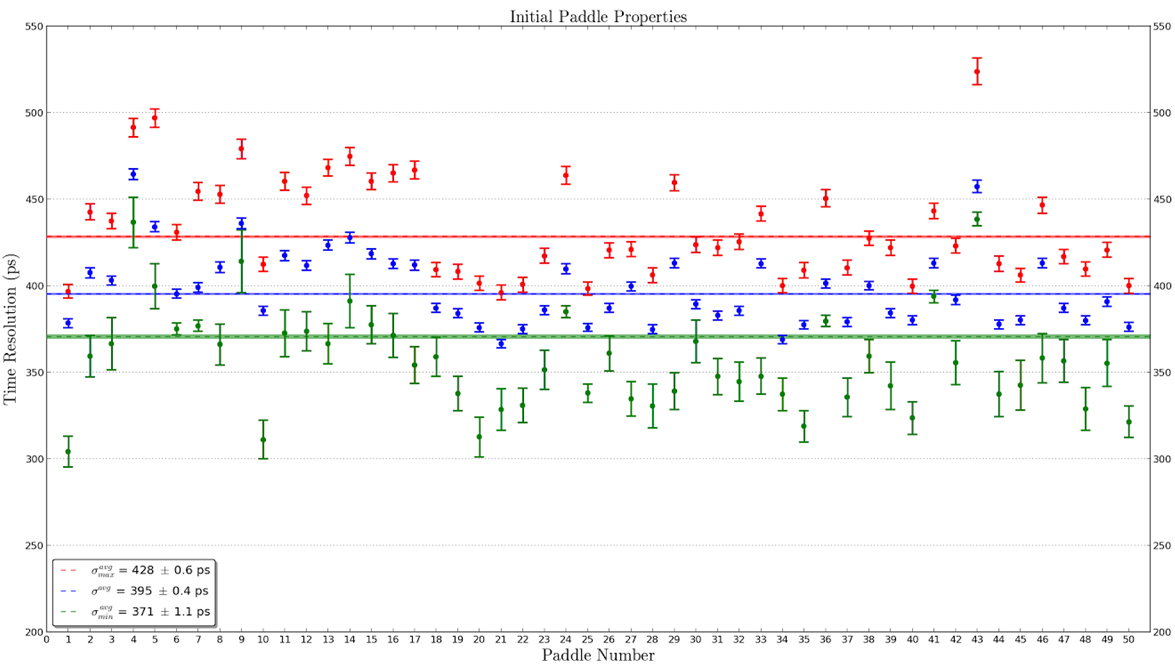
\includegraphics[width=1.0\columnwidth]{fabrication/figs/Initial_Paddle_Prop_UW}
	\caption[Coarse time resolution measurements prior to polishing]{Coarse time resolution measurements prior to polishing. Paddle number is on the x-axis and time resolution in ns is on the y-axis. The red points are the resolutions in the bend region, the blue points are the weighted average of the three measurements, and the green points are the resolutions at the tip of the nose.  The horizontal lines are the weighted averages of the individual measurements.}
	\label{fig:Initial_Paddle_Prop_UW}
\end{figure}
On average the 50 paddles did not meet the design resolution of 350 ps.

To polish the machined scintillator surfaces, Buehler Micropolish II deagglomerated $\mathrm{0.3\ \mu m}$ alumina suspension was utilized\cite{buehler}.  The polishing suspension was diluted with a 5:1 ratio of de-ionized $\mathrm{H_{2}O}$ to alumina and applied to a cold, wet $6'' \times 0.5''$ Caswell Canton flannel buffing wheel\cite{caswell} operated at $\mathrm{<1500~RPMs}$. All surfaces of the scintillators were carefully buffed until all large, uniform surface defects were removed. In order to eliminate small, localized surface defects hand polishing with a soft NOVUS premium Polish Mate microfilament cloth\cite{novus} and diluted polishing suspension was applied.  These polishing procedures made the scintillators void of virtually all scratches and surface defects.

Once the appropriate polishing procedures had been developed and implemented the surface quality was greatly improved as can be seen in Fig.~\ref{fig:polshing_effects} which illustrates the same scintillator paddle before and after polishing.
\begin{figure}[!htb]
	\centering
	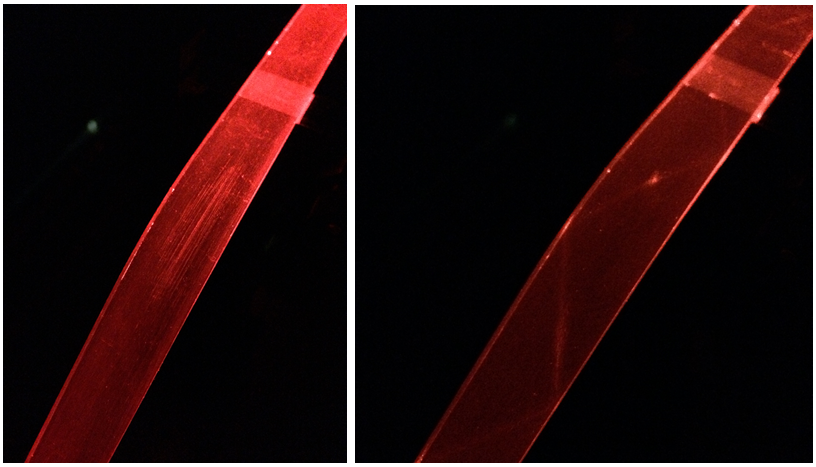
\includegraphics[width=1.0\columnwidth]{fabrication/figs/polshing_effects}
	\caption[Effects of polishing scintillators]{Effects of polishing scintillators. Left: non-diffuse laser incident on an edge, before polishing, at the upstream end of the straight section. Right: non-diffuse laser incident on the same edge, after polishing, at the upstream end of the straight section.}
	\label{fig:polshing_effects}
\end{figure}
A red laser beam was shone into the scintillator medium from the upstream end aimed at one edge so that the total internal reflection towards the tip of the nose was visible.  The unpolished scintillator had such poor surface quality that the reflections in the bend region could not be seen due to the multiple scattering of light at the scintillator boundaries.  However, the reflections in the polished scintillator can clearly be seen traversing down through the nose region.

Once the scintillators were polished, their performance was remeasured so that a quantitative measure of the polishing effects were understood.  The measurements were performed in an identical manner outlined above and the pre-polished results were illustrated in Fig.~\ref{fig:Initial_Paddle_Prop_UW}. As expected, the time resolutions were greatly improved as seen in Fig.~\ref{fig:Polished_Paddle_Prop_UW}.
\begin{figure}[!htb]
	\centering
	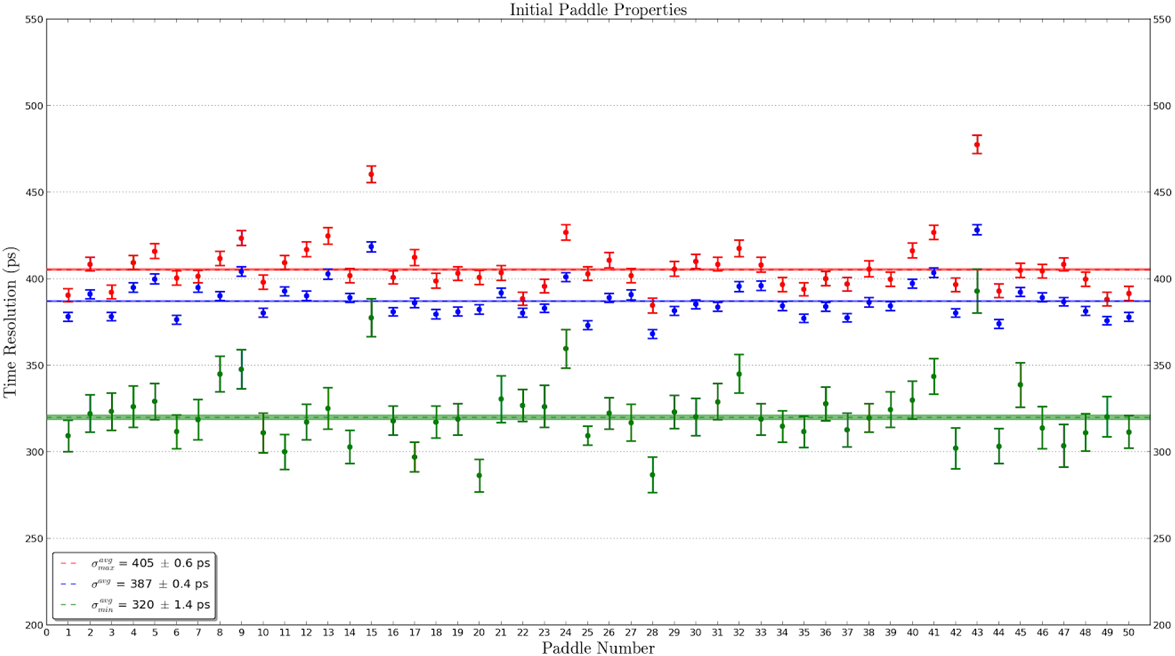
\includegraphics[width=1.0\columnwidth]{fabrication/figs/Polished_Paddle_Prop_UW}
	\caption[Coarse time resolution measurements after polishing]{Coarse time resolution measurements after polishing. The details are identical to Fig.~\ref{fig:Initial_Paddle_Prop_UW}}
	\label{fig:Polished_Paddle_Prop_UW}
\end{figure}
On average, at the tip of the nose, the scintillators exhibited a $\approx15\%$ improvement in time resolution.  Moreover, there was a substantial reduction in erratic fluctuations in performance.

\subsection{Testing Machined Scintillator Paddles} \label{sec:fab_test}

Each of the 50 machined scintillators were tested to study light output and time resolution.  They were measured in an identical manner utilizing a custom fabricated test stand shown in Fig. \ref{fig:test_stand_model}. The test stand allows each scintillator paddle to be measured in an identical and reproducible fashion.  There exist 12 precise locations in which a $^{90}Sr$ source and trigger PMT can be placed so that each of the 50 scintillators are tested at the same locations.  More specifically 4 locations in the straight section, 3 in the bend, and 5 in the nose were tested.
\begin{figure}[!htb]
	\centering
	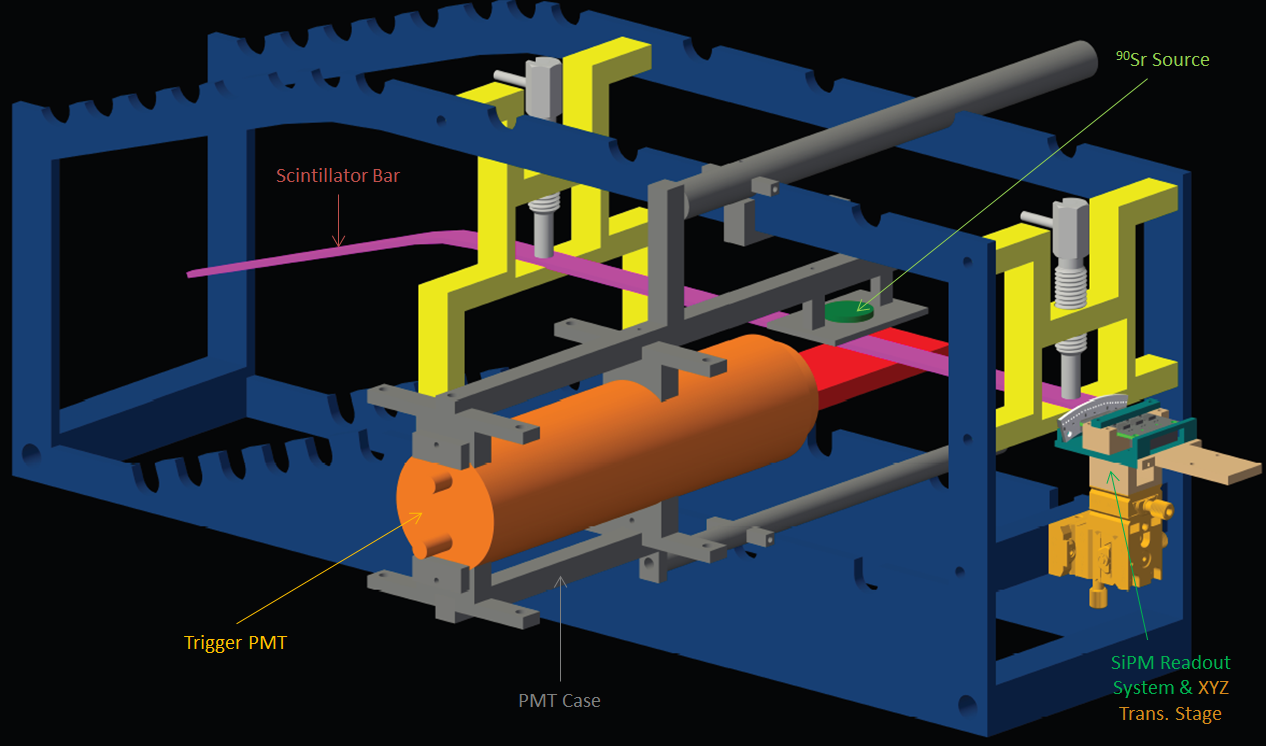
\includegraphics[width=1.0\columnwidth]{fabrication/figs/test_stand_model}
	\caption[CAD Drawing of custom test stand]{CAD Drawing of custom test stand.  The test stand was used in the misalignment studies.}
	\label{fig:test_stand_model}
\end{figure}
